%%
%% Dokumentenart
%%
\NeedsTeXFormat{LaTeX2e}
\documentclass[
    a4paper,
    10pt,
    bibliography=totoc,
    twoside,
    openright,
    numbers=noenddot,
    headings=normal,
    DIV=9,
    parskip
    %,draft
]{scrbook}


%%
%% Unterstützung für deutsche Sprache, Umlaute etc.
%%
\usepackage[utf8]{inputenc}
\usepackage[T1]{fontenc}
\usepackage[ngerman]{babel}
\usepackage[babel,german=quotes]{csquotes}


%%
%% Diverse Pakete
%%
\usepackage{scrhack}
\usepackage{graphicx}
\usepackage{verbatim}
\usepackage{tabularx}
\usepackage{subfigure}
\usepackage{url}
\usepackage{color}
\usepackage{amssymb}
\usepackage{amsmath}
\usepackage{amsthm}
\usepackage{setspace}
\usepackage{listings}
\usepackage{colortbl}
%\usepackage{showframe} % Seitenspiegel anzeigen
\usepackage{microtype}
\usepackage{hyperref} % muss letztes Paket in der Liste sein


%%
%% hier Namen etc. einsetzen
%%
\newcommand{\fullname}{Vorname Nachname}
\newcommand{\email}{vorname.nachname@uni-ulm.de}
\newcommand{\titel}{Ein sehr langer Titel, der sogar über mehrere Zeilen geht:
Wie man noch längere Titel macht}
\newcommand{\jahr}{2012}
\newcommand{\matnr}{123456}
\newcommand{\gutachterA}{Prof.\ Dr.\ Streng Geheim}
\newcommand{\gutachterB}{Prof.\ Dr.\ Un Leserlich}
\newcommand{\betreuer}{Betreuername}
\newcommand{\fakultaet}{Ingenieurwissenschaften\\und Informatik}
%\newcommand{\fakultaet}{Mathematik und\\Wirtschaftswissenschaften}
%\newcommand{\fakultaet}{Naturwissenschaften}
%\newcommand{\fakultaet}{Medizin}
\newcommand{\institut}{Institut für Irgendetwas}
\newcommand{\arbeit}{Diplomarbeit}
%\newcommand{\arbeit}{Bachelorarbeit}


%%
%% Setzt Autor und Titel in den Metadaten des erzeugten Dokumentes
%%
\pdfinfo{
    /Author (\fullname)
    /Title (\titel)
    /Producer (pdfeTex 3.14159-1.30.6-2.2)
    /Keywords ()
}
\hypersetup{
    pdftitle=\titel,
    pdfauthor=\fullname,
    pdfsubject={\arbeit},
    pdfproducer={pdfeTex 3.14159-1.30.6-2.2},
    colorlinks=false,
    pdfborder=0 0 0
}


%%
%% Tiefe, bis zu der Überschriften in das Inhaltsverzeichnis kommen
%%
\setcounter{tocdepth}{3}


%%
%% Verhindert überhängende Absatzteile
%%
\clubpenalty10000
\widowpenalty10000
\displaywidowpenalty=10000


%%
%% Einstellungen für Codelistings
%%
\lstset{
    language=Java,
    showstringspaces=false,
    frame=single,
    numbers=left,
    basicstyle=\ttfamily,
    numberstyle=\tiny
}


%%
%% Formatierung des Literaturverzeichnisses
%%
\bibliographystyle{plaindin} % Nummern und alphabetisch sortiert
%\bibliographystyle{alphadin} % Buchstaben und sortiert
%\bibliographystyle{abbrvdin} % Nummern und abgekürzte Namen
%\bibliographystyle{unsrtdin} % Nummern und unsortiert


%%
%% Eigene Makros
%%
\newcommand{\FIXME}[1]{\colorbox{yellow}{\bf FIXME: #1}}


%%
%% Eigene Farben
%%
\definecolor{Gray}{rgb}{0.80784, 0.86667, 0.90196} %dunkelblau
\definecolor{Lightgray}{rgb}{0.9176, 0.95, 0.95686} %hellblau
\definecolor{Akzent}{rgb}{0.6627, 0.63529, 0.55294} %akzentfarbe


%%
%% Liniendicke in Tabellen etc.
%%
\setlength{\arrayrulewidth}{0.1pt}


%%
%% Schriftarten
%%
\renewcommand{\sfdefault}{phv}
\renewcommand{\rmdefault}{phv}
\renewcommand{\ttdefault}{pcr}
\KOMAoptions{DIV=last}


%%
%% Seitenlayout
%%
\pagestyle{headings}


%%
%% Trennungsregeln
%%
\hyphenation{Sil-ben-trenn-ung}


%%
%% Schönere Bullets bei Aufzählungen
%%
\renewcommand{\labelitemi}{$\bullet$}
\renewcommand{\labelitemii}{$\circ$}
\renewcommand{\labelitemiii}{$\cdot$}


%%
%% Beginn des eigentlichen Dokumentes
%%
\begin{document}


%%
%% Vorspann
%%
\frontmatter


%%
%% Titelseite
%%
\thispagestyle{empty}
\begin{addmargin*}[4mm]{-32mm}


\includegraphics[height=1.8cm]{images/unilogo_bild}
\hfill

\includegraphics[height=1.8cm]{images/unilogo_wort}
\vspace*{2.1em}

{\footnotesize
{\bfseries Universität Ulm} \textbar ~89069 Ulm \textbar ~Germany
\hfill\parbox[t]{42mm}{\bfseries Fakultät für\\
\fakultaet\\
\mdseries \institut}
\vspace*{2cm}

\parbox{140mm}{\bfseries \huge \titel}

{\footnotesize \arbeit{} an der Universität Ulm}
\vspace*{4em}

{\footnotesize
{\bfseries Vorgelegt von:}\\
\fullname\\\email\\[2em]
{\bfseries Gutachter:}\\
\gutachterA\\
\gutachterB\\[2em]
{\bfseries Betreuer:}\\
\betreuer
\\[1.5em]
\jahr}
}
\end{addmargin*}


%%
%% Impressum
%%
\clearpage
\thispagestyle{empty}
{ \small
  \flushleft
  „\titel“\\
  Fassung vom \today \\ \vfill
  \textsc{Danksagungen:} \FIXME{Danksagungen} \\ \vspace{1cm}
  Bei der Erstellung dieser \arbeit{} wurde ausschließlich freie Software eingesetzt: \\
  \begin{figure}[ht]
  	\subfigure{
\includegraphics[height=1cm]{images/sw/ubuntu}}
  	\hspace{0.5cm} 
  	\subfigure{
\includegraphics[height=1cm]{images/sw/texmaker}}
  	\hspace{0.5cm} 
  	\subfigure{
\includegraphics[height=1cm]{images/sw/inkscape}}
  	\hspace{0.5cm} 
  	\subfigure{
\includegraphics[height=1cm]{images/sw/subversion}}
  	\hspace{0.5cm} 
  	\subfigure{
\includegraphics[height=1cm]{images/sw/jabref}}
  	\hspace{0.5cm} 
  	\subfigure{
\includegraphics[height=1cm]{images/sw/firefox}}
  	\hspace{0.5cm} 
  	\subfigure{
\includegraphics[height=1cm]{images/sw/evince}}
  \end{figure}  
  
  \vspace{1cm}
  Satz: PDF-\LaTeXe \\
  Druck: \FIXME{Druck} \\ \vspace{1cm}
  \copyright~\jahr~\fullname\\[0.5em]
% Falls keine Lizenz gewünscht wird bitte den folgenden Text entfernen.
% Die Lizenz erlaubt es zu nichtkommerziellen Zwecken die Arbeit zu
% vervielfältigen und Kopien zu machen. Dabei muss aber immer der Autor
% angegeben werden. Eine kommerzielle Verwertung ist für den Autor
% weiter möglich.
Dieses Werk ist unter der Creative Commons Attribution-NonCommercial-ShareAlike 3.0 Germany License lizensiert: \url{http://creativecommons.org/licenses/by-nc-sa/3.0/de/}\\
  Satz: PDF-\LaTeXe
}


%%
%% Inhaltsverzeichnis
%%
\setstretch{1.4}
\tableofcontents


%%
%% Hauptteil
%%
\mainmatter
\chapter{Einleitung}

Diese kleine Einleitung soll dem Nutzer helfen selbst die eigene Arbeit mit \LaTeX{} zu schreiben. Sie enthält zu den wichtigsten Themen Beispiele.


\section{Struktur}

Für diese Arbeit lassen sich als Überschriften die Überschriften in verschiedenen Stufen verwenden.

\begin{verbatim}
    \chapter{Einleitung}
    \section{Struktur}
    \subsection{}
    \subsubsection{}
\end{verbatim}

Allerdings sollte man sich überlegen, ob man wirklich bis zur Stufe \verb|subsubsection| Überschriften benötigt.



\section{Illustrationen}


\subsection{Bilder}

Bilder kann man natürlich auch in Arbeiten integrieren. Für Fotos und ähnliches unterstützt PDF-\LaTeX{} direkt \verb|jpg| und \verb|png|, ansonsten empfiehlt es sich Vektorgrafiken zu verwenden und diese als \verb|pdf| zu speichern. Sollte ein Bild einmal zu viel weißen Raum um sich haben, so kann man mit dem Werkzeug \verb|pdfcrop| das Bild automatisch ausschneiden\cite{pdfcrop}.

\begin{figure}[ht]
    \centering
    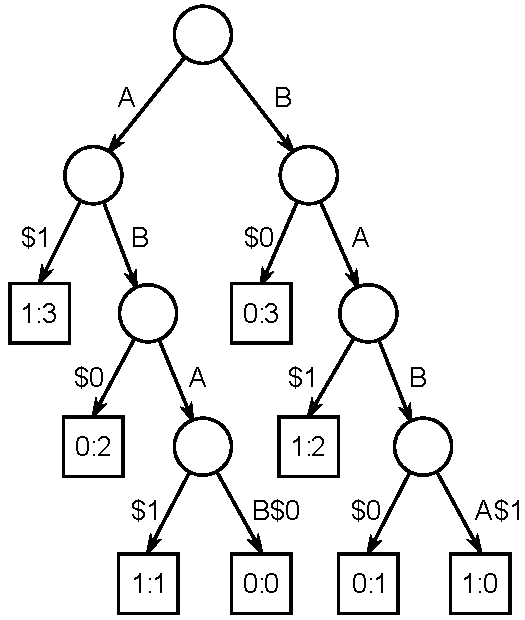
\includegraphics[width=.4\textwidth]{images/Suffix_tree_ABAB_BABA}
    \caption{\label{anker}Bechreibung des Bilds}
\end{figure}

Mit Hilfe eines Labels kann man sich dann im Text auf diese Grafik (\ref{anker}) beziehen. 

\begin{figure}[ht]
    \centering
    \subfigure[Ein fettes u]{
        
\includegraphics[width=0.2\linewidth]{images/a}
        \label{subfigurebsp:a}
    }
    \hspace{1cm}
    \subfigure[Ein dünneres u]{
        
\includegraphics[width=0.2\linewidth]{images/b}
        \label{subfigurebsp:b}
    }
    \caption{Die \emph{u}s aus der Wortmarke}
\end{figure}

Durch \verb|subfigure| lassen sich auch zwei kleine Bilder nebeneinander setzen. In Abbildung \ref{subfigurebsp:a} ist ein fettes u auf der linken und in \ref{subfigurebsp:b} ein dünneres auf der rechten Seite zu sehen.


\subsection{Tabellen}

Hier nur ein kurzes Beispiel, in jedem \LaTeX{} Buch finden sich gute Anleitungen zum Erstellen von Tabellen.

\begin{table}[h]
    \centering
    \begin{tabular}{|l|l|l|}
        A & B & C \\
        \hline
        x & x & x \\
        x & x & x
    \end{tabular}
\end{table}


\subsection{Formeln}

Mathematische Formeln lassen sich als Umgebung mit \verb|\begin{math}| und \verb|\end{math}| erzeugen, es gibt aber auch eine abgekürzte Schreibweise mit \verb|\( Formel \)| wobei die Formel dann im laufenden Text bleibt. Die kürzeste Form ist mit zwei \verb|$| um die Formel, z.B.~so Wasser ist H$_2$O.

Mit der Schreibweise \verb|\[ Formel \]| wird die Formel mittig auf einer neuen Zeile gesetzt, z.B.

\[y = x^2 \]

Dies ist die Kurzform der Umgebung \verb|equation|, mit der die Gleichung auch nummeriert wird. 

\begin{equation}
    x_{1,2} = \frac{-b\pm\sqrt{b^2-4ac}}{2a}
    \label{mitternachtsformel}
\end{equation}

Wenn wir z.B.~über die beliebte Mitternachtsformel (Gleichung \ref{mitternachtsformel}) schreiben wollen lässt sich diese also wie ein Bild referenzieren.



\subsection{Quellcode}

Quellcode und ähnlich zu formatierende Texte können mit \verb|verbatim| in einer Umgebung gesetzt werden.

\begin{verbatim}
Dieser Text ist in Schreibmaschinenschrift
\end{verbatim}

Schöner geht es mit dem \verb|listings|-Paket, das Quelltext auch entsprechend formatiert. Dazu kann man in der Präambel die Sprache angeben in der Quelltexte sind.

\begin{lstlisting}
public class Hello {
    public static void main(String[] args) {
        System.out.println("Hello World");
    }
}
\end{lstlisting}

Im Text gibt man Wörter am Besten als \verb|\verb##| an, dabei erwartet \LaTeX{} zweimal das gleiche Zeichen als Begrenzung. Im Beispiel ist dies die Raute \verb|#|, man kann aber ein anderes Zeichen nehmen, je nachdem was im zu druckenden Wort an Zeichen vorkommt.



\section{Text}

Text kann mit dem Befehl \verb|\emph{}| \emph{hervorgehoben} werden. Falls in einem Satz ein Punkt vorkommt macht man vor ihm kein Leerzeichen sondern einen Backslash (\verb|\|), denn dann fügt \LaTeX{} den korrekten Abstand ein. Zwischen manche Abkürzungen wie z.\,B.\ fügt man zusätzlich \verb|\,| ein, um einen schmalen Abstand zu erzeugen.

\begin{verbatim}
z.\,B.\ so
\end{verbatim}

In der Präambel von \verb|arbeit.tex| gibt es den Befehl \verb|hypenation|, der zur Silbentrennung da ist. \LaTeX hat eine eingebaute Silbentrennung, die jedoch bei manchen Wörtern falsch trennt. Damit diese Worte korrekt getrennt werden gibt man sie dann mit dem Befehl an\footnote{Das Wort \emph{Silbentrennung} ist hier das Beispiel}.

Fußnoten werden mit dem Befehl \verb|footnote| gemacht\footnote{Wie man schon im vorherigen Absatz sehen konnte.}.

In wissenschaftlichen Arbeiten muss man des öfteren andere Arbeiten zitieren. Dazu nutzt man den Befehl \verb|\cite{name}|. In eckigen Klammern kann man noch die Seitenzahl angeben, falls notwendig. Der Name ist ein Schlüssel aus der Datei \verb|bibliography.bib| \cite[S.\ 10]{kopka}. Falls einmal ein Werk indirekt zu einem Teil der Arbeit beigetragen hat kann man es auch mit \verb|nocite| angeben, dann landet es in der Literaturliste, aber nicht direkt im Text.


\subsection{Aufzählungen}

\begin{itemize}
    \item  Hier
    \item  stehen
    \item  Sachen
    \begin{itemize}
        \item  die
        \item  sogar
        \item  eingerückt werden können.
    \end{itemize}
\end{itemize}


\subsection{TeX-Tricks}

Ein geschütztes Leerzeichen an dem nicht umgebrochen wird, setzt man mit \verb!~!.

Dank UTF8 gehen auch Anführungszeichen toll: „“

Unter \emph{Windows} und \emph{Linux} können die Anführungszeichen mit \texttt{AltGr+V} und \texttt{AltGr+B} eingegeben werden. Unter \emph{OS X} drückt man \texttt{Alt+\^{}} und \texttt{Alt+2}.

In manchen Editoren klappt das leider nicht. Dort kann man entweder manuell deutsche Anführungszeichen mit \verb!\glqq! und \verb!\grqq! setzen oder mit \verb!\enquote{Text}! die Art der Zeichen für das ganze Dokument im Header anpassen.


\subsection{Weiterführendes}

Zum Schluß sei auf die Vielzahl an Büchern zu \LaTeX{} verwiesen. In jeder Bibliothek wird sich eine Einführung finden, in der dann weitere Themen wie mathematische Formeln, Aufbau von Briefen und viele nützliche Erweiterungen besprochen werden.


% hier weitere Kapitel einbinden


%%
%% Anhänge
%%
\appendix
\chapter{Quelltexte}

In diesem Anhang sind einige wichtige Quelltexte aufgeführt.

\begin{lstlisting}
public class Hello {
    public static void main(String[] args) {
        System.out.println("Hello World");
    }
}
\end{lstlisting}



%%
%% Nachspann
%%
\backmatter


%%
%% Literaturverzeichnis
%%
\bibliography{bibliography}


%%
%% Versicherung
%%
\cleardoublepage
\thispagestyle{empty}

Name: \fullname \hfill Matrikelnummer: \matnr \vspace{2cm}

\minisec{Erklärung}

Ich erkläre, dass ich die Arbeit selbständig verfasst und keine anderen als die angegebenen Quellen und Hilfsmittel verwendet habe.\vspace{2cm}

Ulm, den \dotfill

\hspace{10cm} {\footnotesize \fullname}
\end{document}
